\documentclass{article}

% if you need to pass options to natbib, use, e.g.:
%     \PassOptionsToPackage{numbers, compress}{natbib}
% before loading neurips_2020

% ready for submission
% \usepackage{neurips_2020}

% to compile a preprint version, e.g., for submission to arXiv, add add the
% [preprint] option:
%     \usepackage[preprint]{neurips_2020}

% to compile a camera-ready version, add the [final] option, e.g.:
    \usepackage[final]{neurips_2020}

% to avoid loading the natbib package, add option nonatbib:
     % \usepackage[nonatbib]{neurips_2020}

\usepackage[utf8]{inputenc} % allow utf-8 input
\usepackage[T1]{fontenc}    % use 8-bit T1 fonts
\usepackage{hyperref}       % hyperlinks
\usepackage{url}            % simple URL typesetting
\usepackage{booktabs}       % professional-quality tables
\usepackage{amsfonts}       % blackboard math symbols
\usepackage{nicefrac}       % compact symbols for 1/2, etc.
\usepackage{microtype}      % microtypography


%% Customized package by Mao Song
\usepackage{graphicx}
\usepackage{amsthm}
\usepackage{amsmath}
\theoremstyle{definition}
\newtheorem{solution}{Solution}
\newtheorem{remark}{Remark}

\title{Homework 2 for SI211: Numerical Analysis}

% The \author macro works with any number of authors. There are two commands
% used to separate the names and addresses of multiple authors: \And and \AND.
%
% Using \And between authors leaves it to LaTeX to determine where to break the
% lines. Using \AND forces a line break at that point. So, if LaTeX puts 3 of 4
% authors names on the first line, and the last on the second line, try using
% \AND instead of \And before the third author name.

\author{%
  {Mao Song} \\
  SIST\\
  ShanghaiTech University\\
  Student ID: 2019233134 \\
  \texttt{maosong@shanghaitech.edu.cn} \\
}

\begin{document}

\maketitle

\begin{abstract}
  This is the solution for Homework 2 of SI211: Numerical Analysis, which is taught by Boris Houska.
\end{abstract}

\section{Jacobian Matrix}
\begin{solution}
  The Jacobian matrix of $f(x)$ is
  \begin{equation}
    J=\begin{bmatrix}
      2x_1x_2+x_2^2& x_1^2+2x_1x_2\\
      2x_1+x_2& x_1
    \end{bmatrix}
  \end{equation}
  subsitute $x=(1,2)^T$ into the above equation, we have
  \begin{equation}
    J|_{(1,2)^T}=\begin{bmatrix}
      8& 5\\
      4& 1
    \end{bmatrix}
  \end{equation}
\end{solution}

\section{Polynomial interpolation}
\begin{solution}
  Since $p(-1)=f(-1)=6$, $p(2)=f(2)=12$, $p(4)=f(4)=66$, we have
  \begin{align}
    a_0-a_1-a_2&=6\\
    a_0+2a_1+8a_2&=12\\
    a_0+4a_1+64a_2&=66
  \end{align}
  rewrite it as the matrix form
  \begin{equation}
    \begin{bmatrix}
      1& -1& -1\\
      1&  2& 8\\
      1& 4& 64&
    \end{bmatrix}\begin{bmatrix}
      a_0\\
      a_1\\
      a_2
    \end{bmatrix}=\begin{bmatrix}
      6\\
      12\\
      66
    \end{bmatrix}\Rightarrow\begin{bmatrix}
      a_0\\
      a_1\\
      a_2
    \end{bmatrix}=\begin{bmatrix}
      6\\
      -1\\
      1
    \end{bmatrix}
  \end{equation}
\end{solution}

\section{Interpolation with rational functions}
\begin{solution}
  We have that $q(-2)=f(-2)=-6$, $p(-1)=f(-1)=-3$, $p(1)=f(1)=5$, $p(2)=f(2)=10$, which is the same as
  \begin{equation}
    \begin{bmatrix}
      -1/2& 1& -2& 4\\
      -1& 1& -1& 1\\
      1 & 1 & 1& 1\\
      1/2& 1 & 2 & 4
    \end{bmatrix}\begin{bmatrix}
      a_{-1}\\
      a_0\\
      a_1\\
      a_2
    \end{bmatrix}=\begin{bmatrix}
      -6\\
      -3\\
      5\\
      10
    \end{bmatrix}
  \end{equation}
  of which the solution is 
  \begin{equation}
    \begin{bmatrix}
      a_{-1}\\
      a_0\\
      a_1\\
      a_2
    \end{bmatrix}=\begin{bmatrix}
      0\\
      2/3\\
      4\\
      1/3
    \end{bmatrix}
  \end{equation}
\end{solution}


\section{Hermite interpolation}
\begin{solution}
From the initial condition, $n=1$. We first compute the Lagrange polynomials and their derivatives. This gives (We use the notation $x_0=1$ and $x_1=2$ for simplicity.)
\begin{align*}
L_{1,0}(x)&=\frac{x-x_1}{x_0-x_1}=-(x-2),\quad  L_{1,0}'(x)=-1\\
L_{1,1}(x)&=\frac{x-x_0}{x_1-x_0}=x-1,\quad  L_{1,1}'(x)=1
\end{align*}
The polynomials $H_{1,0}(x), H_{1,1}(x)$ and $\hat{H}_{1,0}(x), \hat{H}_{1,1}(x)$ are then
\begin{align*}
H_{1,0}(x)&=[1-2(x-x_0)L'_{1,0}(x)]L_{1,0}^2(x)=(2x-1)(x-2)^2   \\
H_{1,1}(x)&=[1-2(x-x_1)L'_{1,1}(x)]L_{1,1}^2(x)=(-2x+5)(x-1)^2    \\
\hat{H}_{1,0}(x)&=(x-x_0)L_{1,0}^2(x)=(x-1)(x-2)^2    \\
\hat{H}_{1,1}(x)&=(x-x_1)L_{1,1}^2(x)=(x-2)(x-1)^2   \\
\end{align*}
Finally,
\begin{align*}
H_3(x)&=\left[p(x_0)H_{1,0}(x)+p(x_1)H_{1,1}(x)\right]+\left[p'(x_0)\hat{H}_{1,0}(x)+p'(x_1)\hat{H}_{1,1}(x)\right]\\
&=H_{1,0}(x)+2H_{1,1}(x)+2\hat{H}_{1,0}(x)+4\hat{H}_{1,1}(x)\\
&=(2x-1)(x-2)^2+2(-2x+5)(x-1)^2+2(x-1)(x-2)^2+4(x-2)(x-1)^2\\
&=(4x-3)(x-2)^2+2(x-1)^2\\
&=4x^3-17x^2+24x-10
\end{align*}

\end{solution}



\section{Polynomial Approximation error}
\begin{solution}
  The results are shown as follows:
    \begin{figure}[ht]
      \label{Fig:solution_to_problem5_1}  
      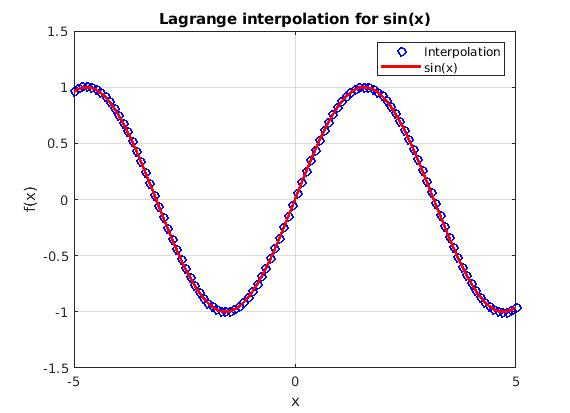
\includegraphics[width=0.8\textwidth]{plot_5_1.jpg}
      \centering
      \caption{The interpolation for $\sin(x)$}
    \end{figure}

    \begin{figure}[ht]
      \label{Fig:solution_to_problem3}
      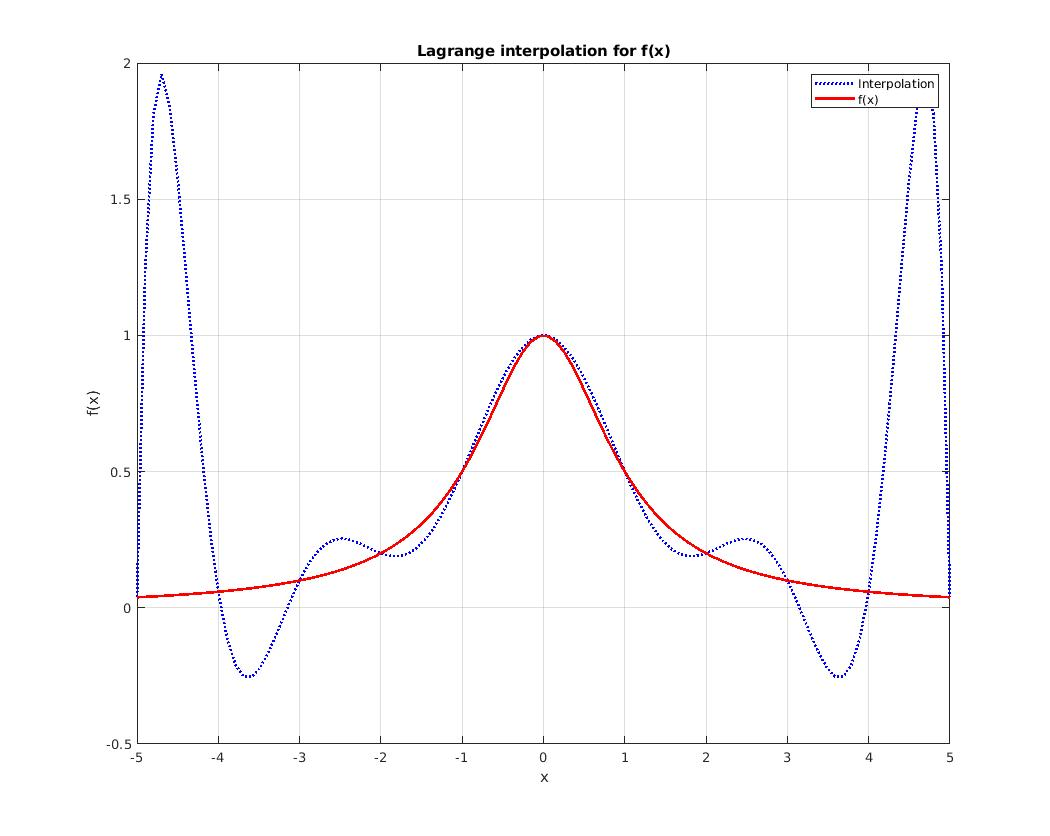
\includegraphics[width=0.8\textwidth]{plot_5_2.jpg}
      \centering
      \caption{The interpolation for $f(x)=1/(1+x^2)$}
    \end{figure}

    Now we analysis the approximation error. By Theorem 3.3 of \emph{Numerical Analysis, 9th ed}. We have
    \begin{equation}
      f(x)=P(x)+\frac{f^{(11)}(\xi(x))}{11!}(x+5)\cdots(x-5)
    \end{equation}
    where $P(x)$ is the Lagrange interpolation polynomial, $\xi(x)\in[-5,5]$.
    \begin{enumerate}
      \item $f(x)=\sin(x)$. We have
      \begin{equation}
        f^{(11)}(x)=-\cos(x)
      \end{equation}
      and 
      \begin{align*}
      \frac{f^{(11)}(\xi(x))}{11!}(x+5)\cdots(x-5)&=\frac{-\cos(\xi(x))}{11!}(x+5)\cdots(x-5)
      \end{align*}
      The maximal value of $\cos(\xi(x))$ on the interval $[-5,5]$ is $1$. Define $g(x)=(x+5)\cdots(x-5)$, $x\in[-5,5]$.
      Since the mximum value of $g(x)$ is attained at $x^*\approx-4.71458$, and $g(x^*)\approx416614$ and $g(x)$ is an odd function. Thus
      \begin{equation}
        |g(x)|\leq 416620, x\in[-5,5]
      \end{equation}
      Now we have
      \begin{equation}
        |\frac{-\cos(\xi(x))}{11!}(x+5)\cdots(x-5)|\leq \frac{416620}{11!}\approx 0.01
      \end{equation}
      which is consistent with the plot.

      \item $f(x)=1/(1+x^2)$. We use Mathematica to obtain an upper bound for $|f^{(11)}(\xi(x))|$:
      \begin{equation}
        |f^{(11)}(\xi(x))|\leq |f^{(11)}(0.12)|\leq 3.6\times 10^7
      \end{equation}

      \begin{equation}
        |\frac{f^{(11)}(\xi(x))}{11!}(x-x_0)\cdots(x-x_{10})|\leq \frac{416620\times 3.6\times 10^7}{11!}\approx 3.6\times 10^5
      \end{equation}
      The bound indicates that the Lagrange interpolation method is unstable for $f(x)=1/(1+x^2)$. Actually, as $n$ increases, the oscillations get even larger. The interpolation polynomial $P(x)$ doesn't converge to $f(x)$ uniformly.
      




    \end{enumerate}
    
\end{solution}






% \subsection{Style}

% Papers to be submitted to NeurIPS 2020 must be prepared according to the
% instructions presented here. Papers may only be up to eight pages long,
% including figures. Additional pages \emph{containing only a section on the broader impact, acknowledgments and/or cited references} are allowed. Papers that exceed eight pages of content will not be reviewed, or in any other way considered for
% presentation at the conference.

% The margins in 2020 are the same as those in 2007, which allow for $\sim$$15\%$
% more words in the paper compared to earlier years.

% Authors are required to use the NeurIPS \LaTeX{} style files obtainable at the
% NeurIPS website as indicated below. Please make sure you use the current files
% and not previous versions. Tweaking the style files may be grounds for
% rejection.

% \subsection{Retrieval of style files}

% The style files for NeurIPS and other conference information are available on
% the World Wide Web at
% \begin{center}
%   \url{http://www.neurips.cc/}
% \end{center}
% The file \verb+neurips_2020.pdf+ contains these instructions and illustrates the
% various formatting requirements your NeurIPS paper must satisfy.

% The only supported style file for NeurIPS 2020 is \verb+neurips_2020.sty+,
% rewritten for \LaTeXe{}.  \textbf{Previous style files for \LaTeX{} 2.09,
%   Microsoft Word, and RTF are no longer supported!}

% The \LaTeX{} style file contains three optional arguments: \verb+final+, which
% creates a camera-ready copy, \verb+preprint+, which creates a preprint for
% submission to, e.g., arXiv, and \verb+nonatbib+, which will not load the
% \verb+natbib+ package for you in case of package clash.

% \paragraph{Preprint option}
% If you wish to post a preprint of your work online, e.g., on arXiv, using the
% NeurIPS style, please use the \verb+preprint+ option. This will create a
% nonanonymized version of your work with the text ``Preprint. Work in progress.''
% in the footer. This version may be distributed as you see fit. Please \textbf{do
%   not} use the \verb+final+ option, which should \textbf{only} be used for
% papers accepted to NeurIPS.

% At submission time, please omit the \verb+final+ and \verb+preprint+
% options. This will anonymize your submission and add line numbers to aid
% review. Please do \emph{not} refer to these line numbers in your paper as they
% will be removed during generation of camera-ready copies.

% The file \verb+neurips_2020.tex+ may be used as a ``shell'' for writing your
% paper. All you have to do is replace the author, title, abstract, and text of
% the paper with your own.

% The formatting instructions contained in these style files are summarized in
% Sections \ref{gen_inst}, \ref{headings}, and \ref{others} below.

% \section{General formatting instructions}
% \label{gen_inst}

% The text must be confined within a rectangle 5.5~inches (33~picas) wide and
% 9~inches (54~picas) long. The left margin is 1.5~inch (9~picas).  Use 10~point
% type with a vertical spacing (leading) of 11~points.  Times New Roman is the
% preferred typeface throughout, and will be selected for you by default.
% Paragraphs are separated by \nicefrac{1}{2}~line space (5.5 points), with no
% indentation.

% The paper title should be 17~point, initial caps/lower case, bold, centered
% between two horizontal rules. The top rule should be 4~points thick and the
% bottom rule should be 1~point thick. Allow \nicefrac{1}{4}~inch space above and
% below the title to rules. All pages should start at 1~inch (6~picas) from the
% top of the page.

% For the final version, authors' names are set in boldface, and each name is
% centered above the corresponding address. The lead author's name is to be listed
% first (left-most), and the co-authors' names (if different address) are set to
% follow. If there is only one co-author, list both author and co-author side by
% side.

% Please pay special attention to the instructions in Section \ref{others}
% regarding figures, tables, acknowledgments, and references.

% \section{Headings: first level}
% \label{headings}

% All headings should be lower case (except for first word and proper nouns),
% flush left, and bold.

% First-level headings should be in 12-point type.

% \subsection{Headings: second level}

% Second-level headings should be in 10-point type.

% \subsubsection{Headings: third level}

% Third-level headings should be in 10-point type.

% \paragraph{Paragraphs}

% There is also a \verb+\paragraph+ command available, which sets the heading in
% bold, flush left, and inline with the text, with the heading followed by 1\,em
% of space.

% \section{Citations, figures, tables, references}
% \label{others}

% These instructions apply to everyone.

% \subsection{Citations within the text}

% The \verb+natbib+ package will be loaded for you by default.  Citations may be
% author/year or numeric, as long as you maintain internal consistency.  As to the
% format of the references themselves, any style is acceptable as long as it is
% used consistently.

% The documentation for \verb+natbib+ may be found at
% \begin{center}
%   \url{http://mirrors.ctan.org/macros/latex/contrib/natbib/natnotes.pdf}
% \end{center}
% Of note is the command \verb+\citet+, which produces citations appropriate for
% use in inline text.  For example,
% \begin{verbatim}
%    \citet{hasselmo} investigated\dots
% \end{verbatim}
% produces
% \begin{quote}
%   Hasselmo, et al.\ (1995) investigated\dots
% \end{quote}

% If you wish to load the \verb+natbib+ package with options, you may add the
% following before loading the \verb+neurips_2020+ package:
% \begin{verbatim}
%    \PassOptionsToPackage{options}{natbib}
% \end{verbatim}

% If \verb+natbib+ clashes with another package you load, you can add the optional
% argument \verb+nonatbib+ when loading the style file:
% \begin{verbatim}
%    \usepackage[nonatbib]{neurips_2020}
% \end{verbatim}

% As submission is double blind, refer to your own published work in the third
% person. That is, use ``In the previous work of Jones et al.\ [4],'' not ``In our
% previous work [4].'' If you cite your other papers that are not widely available
% (e.g., a journal paper under review), use anonymous author names in the
% citation, e.g., an author of the form ``A.\ Anonymous.''

% \subsection{Footnotes}

% Footnotes should be used sparingly.  If you do require a footnote, indicate
% footnotes with a number\footnote{Sample of the first footnote.} in the
% text. Place the footnotes at the bottom of the page on which they appear.
% Precede the footnote with a horizontal rule of 2~inches (12~picas).

% Note that footnotes are properly typeset \emph{after} punctuation
% marks.\footnote{As in this example.}

% \subsection{Figures}

% \begin{figure}
%   \centering
%   \fbox{\rule[-.5cm]{0cm}{4cm} \rule[-.5cm]{4cm}{0cm}}
%   \caption{Sample figure caption.}
% \end{figure}

% All artwork must be neat, clean, and legible. Lines should be dark enough for
% purposes of reproduction. The figure number and caption always appear after the
% figure. Place one line space before the figure caption and one line space after
% the figure. The figure caption should be lower case (except for first word and
% proper nouns); figures are numbered consecutively.

% You may use color figures.  However, it is best for the figure captions and the
% paper body to be legible if the paper is printed in either black/white or in
% color.

% \subsection{Tables}

% All tables must be centered, neat, clean and legible.  The table number and
% title always appear before the table.  See Table~\ref{sample-table}.

% Place one line space before the table title, one line space after the
% table title, and one line space after the table. The table title must
% be lower case (except for first word and proper nouns); tables are
% numbered consecutively.

% Note that publication-quality tables \emph{do not contain vertical rules.} We
% strongly suggest the use of the \verb+booktabs+ package, which allows for
% typesetting high-quality, professional tables:
% \begin{center}
%   \url{https://www.ctan.org/pkg/booktabs}
% \end{center}
% This package was used to typeset Table~\ref{sample-table}.

% \begin{table}
%   \caption{Sample table title}
%   \label{sample-table}
%   \centering
%   \begin{tabular}{lll}
%     \toprule
%     \multicolumn{2}{c}{Part}                   \\
%     \cmidrule(r){1-2}
%     Name     & Description     & Size ($\mu$m) \\
%     \midrule
%     Dendrite & Input terminal  & $\sim$100     \\
%     Axon     & Output terminal & $\sim$10      \\
%     Soma     & Cell body       & up to $10^6$  \\
%     \bottomrule
%   \end{tabular}
% \end{table}

% \section{Final instructions}

% Do not change any aspects of the formatting parameters in the style files.  In
% particular, do not modify the width or length of the rectangle the text should
% fit into, and do not change font sizes (except perhaps in the
% \textbf{References} section; see below). Please note that pages should be
% numbered.

% \section{Preparing PDF files}

% Please prepare submission files with paper size ``US Letter,'' and not, for
% example, ``A4.''

% Fonts were the main cause of problems in the past years. Your PDF file must only
% contain Type 1 or Embedded TrueType fonts. Here are a few instructions to
% achieve this.

% \begin{itemize}

% \item You should directly generate PDF files using \verb+pdflatex+.

% \item You can check which fonts a PDF files uses.  In Acrobat Reader, select the
%   menu Files$>$Document Properties$>$Fonts and select Show All Fonts. You can
%   also use the program \verb+pdffonts+ which comes with \verb+xpdf+ and is
%   available out-of-the-box on most Linux machines.

% \item The IEEE has recommendations for generating PDF files whose fonts are also
%   acceptable for NeurIPS. Please see
%   \url{http://www.emfield.org/icuwb2010/downloads/IEEE-PDF-SpecV32.pdf}

% \item \verb+xfig+ "patterned" shapes are implemented with bitmap fonts.  Use
%   "solid" shapes instead.

% \item The \verb+\bbold+ package almost always uses bitmap fonts.  You should use
%   the equivalent AMS Fonts:
% \begin{verbatim}
%    \usepackage{amsfonts}
% \end{verbatim}
% followed by, e.g., \verb+\mathbb{R}+, \verb+\mathbb{N}+, or \verb+\mathbb{C}+
% for $\mathbb{R}$, $\mathbb{N}$ or $\mathbb{C}$.  You can also use the following
% workaround for reals, natural and complex:
% \begin{verbatim}
%    \newcommand{\RR}{I\!\!R} %real numbers
%    \newcommand{\Nat}{I\!\!N} %natural numbers
%    \newcommand{\CC}{I\!\!\!\!C} %complex numbers
% \end{verbatim}
% Note that \verb+amsfonts+ is automatically loaded by the \verb+amssymb+ package.

% \end{itemize}

% If your file contains type 3 fonts or non embedded TrueType fonts, we will ask
% you to fix it.

% \subsection{Margins in \LaTeX{}}

% Most of the margin problems come from figures positioned by hand using
% \verb+\special+ or other commands. We suggest using the command
% \verb+\includegraphics+ from the \verb+graphicx+ package. Always specify the
% figure width as a multiple of the line width as in the example below:
% \begin{verbatim}
%    \usepackage[pdftex]{graphicx} ...
%    \includegraphics[width=0.8\linewidth]{myfile.pdf}
% \end{verbatim}
% See Section 4.4 in the graphics bundle documentation
% (\url{http://mirrors.ctan.org/macros/latex/required/graphics/grfguide.pdf})

% A number of width problems arise when \LaTeX{} cannot properly hyphenate a
% line. Please give LaTeX hyphenation hints using the \verb+\-+ command when
% necessary.


% \section*{Broader Impact}

% Authors are required to include a statement of the broader impact of their work, including its ethical aspects and future societal consequences. 
% Authors should discuss both positive and negative outcomes, if any. For instance, authors should discuss a) 
% who may benefit from this research, b) who may be put at disadvantage from this research, c) what are the consequences of failure of the system, and d) whether the task/method leverages
% biases in the data. If authors believe this is not applicable to them, authors can simply state this.

% Use unnumbered first level headings for this section, which should go at the end of the paper. {\bf Note that this section does not count towards the eight pages of content that are allowed.}

% \begin{ack}
% Use unnumbered first level headings for the acknowledgments. All acknowledgments
% go at the end of the paper before the list of references. Moreover, you are required to declare 
% funding (financial activities supporting the submitted work) and competing interests (related financial activities outside the submitted work). 
% More information about this disclosure can be found at: \url{https://neurips.cc/Conferences/2020/PaperInformation/FundingDisclosure}.


% Do {\bf not} include this section in the anonymized submission, only in the final paper. You can use the \texttt{ack} environment provided in the style file to autmoatically hide this section in the anonymized submission.
% \end{ack}

% \section*{References}

% References follow the acknowledgments. Use unnumbered first-level heading for
% the references. Any choice of citation style is acceptable as long as you are
% consistent. It is permissible to reduce the font size to \verb+small+ (9 point)
% when listing the references.
% {\bf Note that the Reference section does not count towards the eight pages of content that are allowed.}
% \medskip

% \small

% [1] Alexander, J.A.\ \& Mozer, M.C.\ (1995) Template-based algorithms for
% connectionist rule extraction. In G.\ Tesauro, D.S.\ Touretzky and T.K.\ Leen
% (eds.), {\it Advances in Neural Information Processing Systems 7},
% pp.\ 609--616. Cambridge, MA: MIT Press.

% [2] Bower, J.M.\ \& Beeman, D.\ (1995) {\it The Book of GENESIS: Exploring
%   Realistic Neural Models with the GEneral NEural SImulation System.}  New York:
% TELOS/Springer--Verlag.

% [3] Hasselmo, M.E., Schnell, E.\ \& Barkai, E.\ (1995) Dynamics of learning and
% recall at excitatory recurrent synapses and cholinergic modulation in rat
% hippocampal region CA3. {\it Journal of Neuroscience} {\bf 15}(7):5249-5262.

\end{document}
